\documentclass[12pt,a4paper]{article}
\usepackage{amsmath,amsthm,amssymb,mathtools}
\usepackage{tikz}
\usetikzlibrary{arrows.meta,positioning,shapes.geometric,calc,fit,backgrounds}
\usepackage{graphicx}
\usepackage{booktabs,tabularx,multirow}
\usepackage[ruled,vlined,linesnumbered]{algorithm2e}
\usepackage[most]{tcolorbox}
\usepackage{hyperref}
\usepackage[capitalize,noabbrev]{cleveref}
\usepackage[margin=1in]{geometry}
\usepackage{fancyhdr}
\usepackage{enumitem}
\usepackage{xcolor}

%% ── tcolorbox environments ──────────────────────────────────────────────────
\newtcolorbox{keyinsight}[1][]{colback=blue!5!white,colframe=blue!75!black,fonttitle=\bfseries,title=Key Insight,#1}
\newtcolorbox{example}[1][]{colback=green!5!white,colframe=green!75!black,fonttitle=\bfseries,title=Example,#1}
\newtcolorbox{warningbox}[1][]{colback=red!5!white,colframe=red!75!black,fonttitle=\bfseries,title=Warning,#1}

%% ── amsthm environments ─────────────────────────────────────────────────────
\newtheorem{theorem}{Theorem}[section]
\newtheorem{lemma}[theorem]{Lemma}
\newtheorem{definition}{Definition}[section]
\newtheorem{remark}{Remark}[section]

%% ── page style ───────────────────────────────────────────────────────────────
\pagestyle{fancy}
\fancyhf{}
\rhead{Session 06 -- ANN Advanced Concepts \& Backpropagation}
\lhead{Deep Learning Course}
\rfoot{Page \thepage}

\hypersetup{
  colorlinks=true,
  linkcolor=blue!60!black,
  urlcolor=blue!60!black,
  citecolor=green!50!black
}

%% ── convenience macros ───────────────────────────────────────────────────────
\newcommand{\pd}[2]{\frac{\partial #1}{\partial #2}}
\newcommand{\wji}{w_{ji}^{h}}
\newcommand{\wkj}{w_{kj}}
\newcommand{\sho}{s_{j}^{h}}
\newcommand{\sko}{s_{k}^{o}}
\newcommand{\deltak}{\delta_{k}}
\newcommand{\deltajh}{\delta_{j}^{h}}
\newcommand{\xho}{x_{j}^{h}}
\newcommand{\xko}{x_{k}^{o}}

% ─────────────────────────────────────────────────────────────────────────────
\begin{document}

%% ─── TITLE PAGE ──────────────────────────────────────────────────────────────
\begin{titlepage}
  \centering
  \vspace*{2cm}
  {\Huge\bfseries Deep Learning: Session 06\par}
  \vspace{0.5cm}
  {\LARGE ANN Advanced Concepts \& Backpropagation Derivation\par}
  \vspace{1.5cm}
  \rule{\linewidth}{0.4pt}\\[0.4cm]
  {\large
    \textbf{Course:} Deep Learning (IIIT Dharwad)\\[0.3cm]
    \textbf{Deck:} 02-DL-NNIntro (Slides 50--87 of 87)\\[0.3cm]
    \textbf{Video:} \url{https://vimeo.com/1144087053}\\[0.3cm]
    \textbf{Slides:} \url{https://learning.iiitdwd.ac.in/mod/resource/view.php?id=1309}\\[0.3cm]
    \textbf{Duration:} 1\,h\,46\,min\\[0.3cm]
    \textbf{Instructors:} Prof.\ S\,R\,M\,Prasanna \& Dr.\ Sunil Saumya\\[0.3cm]
    \textbf{Date Recorded:} December 6, 2025\\[0.3cm]
    \textbf{Notes Compiled:} March 2, 2026
  }\\[1.0cm]
  \rule{\linewidth}{0.4pt}\\[1.5cm]
  {\large\itshape
    Topics covered: Hard learning problem, differentiable activation functions,
    backpropagation derivation (generalized delta rule), MSE loss, gradient
    descent on the error surface, PyTorch implementation with and without
    Autograd.
  }
  \vfill
\end{titlepage}

%% ─── TABLE OF CONTENTS ───────────────────────────────────────────────────────
\tableofcontents
\newpage

%% =============================================================================
\section{Introduction}
\label{sec:intro}
%% =============================================================================

Session~06 closes the theoretical foundation of feed-forward artificial neural
networks (ANNs) begun in Session~05, working through slides 50--87 of the deck
\texttt{02-DL-NNIntro}.  The session opens with a concise recap of the
\emph{hard learning problem}, explains why a differentiable nonlinear activation
function is necessary for its solution, derives the backpropagation weight-update
rules in full, introduces Mean Squared Error (MSE) as the canonical regression
loss, discusses convex versus non-convex loss surfaces, and concludes with a
live Google Colab implementation in PyTorch --- first coded by hand and then
using PyTorch's built-in Autograd engine.

The overarching message delivered by the instructors is that backpropagation is
not a mysterious black box: it is a straightforward application of the chain
rule of calculus, and every practitioner should be able to derive and implement
it from scratch before relying on library abstractions.

\begin{keyinsight}[title=Session Objective]
Understand \emph{why} differentiable activation functions are essential, derive
the backpropagation update equations from first principles, and verify the
derivation numerically in PyTorch.
\end{keyinsight}

%% =============================================================================
\section{Background and Prerequisites}
\label{sec:background}
%% =============================================================================

\subsection{Single-Layer Perceptron Recap}

A single-layer perceptron (SLP) consists of an input layer of linear units
connected directly to a perceptron (output) layer.  For an input vector
$\mathbf{a} = (a_1, a_2, \ldots, a_I)^{\top}$ and weight matrix $\mathbf{W}$,
the net input and output of neuron $k$ in the output layer are

\begin{align}
  x_k &= \sum_{i=1}^{I} w_{ki}\,a_i + b_k, \label{eq:slp-net}\\
  s_k &= f(x_k), \label{eq:slp-out}
\end{align}

where $f(\cdot)$ is the activation function.  In the original perceptron,
$f$ is the Heaviside step (signum) function.  The \emph{perceptron learning
rule} (delta rule) updates weights as

\begin{equation}
  \Delta w_{ki} = \eta\,(b_k - s_k)\,a_i,
  \label{eq:perceptron-rule}
\end{equation}

where $b_k$ is the desired (target) output, $s_k$ is the actual output, and
$\eta > 0$ is the learning rate.  This rule works because we know the desired
output $b_k$ for every output neuron.

\subsection{Linearly Separable vs.\ Non-Separable Classes}

\begin{definition}[Linear Separability]
\label{def:linear-sep}
A data set $\{(\mathbf{a}^{(p)}, \mathbf{b}^{(p)})\}_{p=1}^{P}$ is said to be
\emph{linearly separable} if there exists a hyperplane that correctly classifies
all patterns.
\end{definition}

The single-layer perceptron can only solve linearly separable problems.  The
canonical counter-example is the XOR function:

\begin{center}
\begin{tabular}{ccc}
  \toprule
  $x_1$ & $x_2$ & XOR \\
  \midrule
  0 & 0 & 0 \\
  0 & 1 & 1 \\
  1 & 0 & 1 \\
  1 & 1 & 0 \\
  \bottomrule
\end{tabular}
\end{center}

No single straight line can separate the two classes $\{(0,0),(1,1)\}$ from
$\{(0,1),(1,0)\}$, so a multi-layer architecture is required.

\subsection{The Three-Layer Feed-Forward Network (Figure 4.12)}
\label{sub:three-layer}

The reference architecture used throughout this session is Figure~4.12 from
B.\ Yegnanarayana, \textit{Artificial Neural Networks}, PHI, New Delhi,
1999.  It is a three-layer feed-forward network with:

\begin{itemize}[noitemsep]
  \item \textbf{Input layer} ($i = 1,\ldots,I$): linear units with outputs
        $a_i$.
  \item \textbf{Hidden layer} ($j = 1,\ldots,J$): nonlinear units with net
        input $\xho$ and output $\sho$.
  \item \textbf{Output layer} ($k = 1,\ldots,K$): nonlinear units with net
        input $\xko$ and output $\sko$.
\end{itemize}

The weight connecting hidden unit~$j$ to input unit~$i$ is $\wji$; the weight
connecting output unit~$k$ to hidden unit~$j$ is $\wkj$.

\cref{fig:three-layer} shows a TikZ reconstruction of this architecture.

%% ─── FIGURE 1: Three-layer network ──────────────────────────────────────────
\begin{figure}[htbp]
\centering
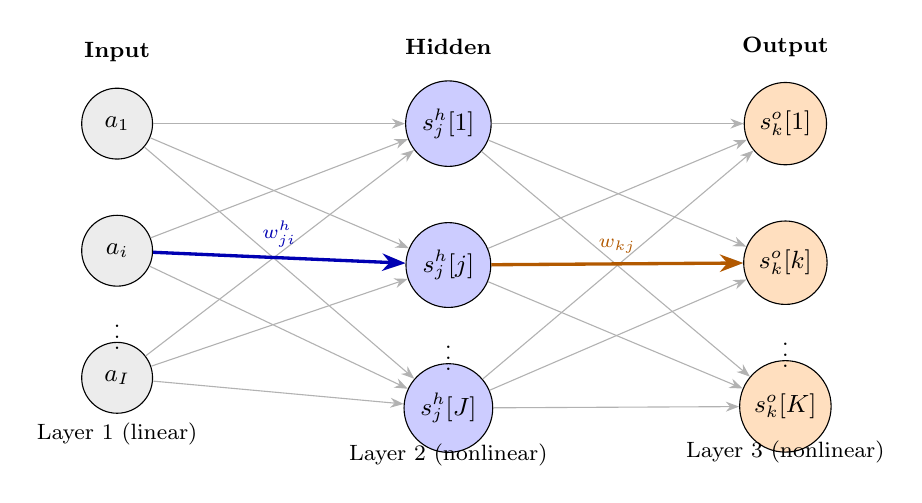
\begin{tikzpicture}[
    node distance=2.2cm and 3.0cm,
    neuron/.style={circle,draw,minimum size=0.9cm,font=\small},
    label/.style={font=\footnotesize},
    >=Stealth
  ]
  %% Input layer
  \node[neuron,fill=gray!15] (i1) {$a_1$};
  \node[neuron,fill=gray!15,below=0.7cm of i1] (i2) {$a_i$};
  \node[neuron,fill=gray!15,below=0.7cm of i2] (i3) {$a_I$};
  \node[label,above=0.2cm of i1] {\textbf{Input}};

  %% Hidden layer
  \node[neuron,fill=blue!20,right=3.2cm of i1] (h1) {$\sho[1]$};
  \node[neuron,fill=blue!20,below=0.7cm of h1] (h2) {$\sho[j]$};
  \node[neuron,fill=blue!20,below=0.7cm of h2] (h3) {$\sho[J]$};
  \node[label,above=0.2cm of h1] {\textbf{Hidden}};

  %% Output layer
  \node[neuron,fill=orange!25,right=3.2cm of h1] (o1) {$\sko[1]$};
  \node[neuron,fill=orange!25,below=0.7cm of o1] (o2) {$\sko[k]$};
  \node[neuron,fill=orange!25,below=0.7cm of o2] (o3) {$\sko[K]$};
  \node[label,above=0.2cm of o1] {\textbf{Output}};

  %% Dots
  \node[label,below=0.15cm of i2]  {$\vdots$};
  \node[label,below=0.15cm of h2]  {$\vdots$};
  \node[label,below=0.15cm of o2]  {$\vdots$};

  %% Input->Hidden edges
  \foreach \src in {i1,i2,i3}{
    \foreach \dst in {h1,h2,h3}{
      \draw[->,gray!60] (\src) -- (\dst);
    }
  }
  %% Label one weight
  \draw[->,very thick,blue!70!black] (i2) -- node[above,font=\scriptsize]{$\wji$} (h2);

  %% Hidden->Output edges
  \foreach \src in {h1,h2,h3}{
    \foreach \dst in {o1,o2,o3}{
      \draw[->,gray!60] (\src) -- (\dst);
    }
  }
  \draw[->,very thick,orange!70!black] (h2) -- node[above,font=\scriptsize]{$\wkj$} (o2);

  %% Layer labels on x-axis
  \node[label,below=1.6cm of i2]  {Layer 1 (linear)};
  \node[label,below=1.6cm of h2]  {Layer 2 (nonlinear)};
  \node[label,below=1.6cm of o2]  {Layer 3 (nonlinear)};
\end{tikzpicture}
\caption{Three-layer feed-forward neural network (Yegnanarayana Fig.\ 4.12
  reconstruction). Highlighted edges carry the weight notation used throughout
  the backpropagation derivation.}
\label{fig:three-layer}
\end{figure}

%% =============================================================================
\section{The Hard Learning Problem}
\label{sec:hard-learning}
%% =============================================================================

\subsection{Two Distinct Difficulties}

Students frequently conflate two different problems that arose in the history of
neural networks.  The instructors in this session took care to distinguish them
explicitly.

\begin{keyinsight}[title=Hard Problem vs.\ Hard Learning Problem]
\begin{description}[labelwidth=4.5cm,leftmargin=!]
  \item[Hard problem] A \emph{representation} difficulty: the data are not
        linearly separable, so a single-layer perceptron cannot solve the task
        (e.g.\ XOR).  Solved by adding hidden layers.
  \item[Hard learning problem] A \emph{training} difficulty: once hidden layers
        are added, we no longer have target outputs for hidden units, so we
        cannot compute the error signal needed to update the hidden-layer
        weights.
\end{description}
\end{keyinsight}

The hard learning problem caused the neural network field to stall for
roughly a decade until the backpropagation learning algorithm was
discovered/popularized in the 1980s.

\subsection{Why the Perceptron Rule Fails for Hidden Layers}

Recall \cref{eq:perceptron-rule}: the weight update requires the error
$(b_k - s_k)$.  For output-layer neurons we know the desired output $b_k$
directly from the training labels, so the error is computable.  For
hidden-layer neuron~$j$, however, we have \textbf{no} desired output --- the
``correct'' hidden-unit activation is not available in any dataset.  Hence
the perceptron rule cannot be applied to $\wji$.

\begin{remark}
\label{rem:why-hidden}
This is precisely why hidden layers are called \emph{hidden}: their targets are
hidden from us.  The backpropagation algorithm circumvents this by propagating
the \emph{output-layer error} backwards through the network to obtain a proxy
error signal for each hidden unit.
\end{remark}

\subsection{The Key Insight Behind Backpropagation}

Hidden unit~$j$ feeds into \emph{all} output neurons $k = 1,\ldots,K$.
Therefore it contributes a fraction of the total output error.  If we can
express the error at hidden unit~$j$ as a weighted sum of the output-layer
errors --- weighted by the connecting weights $\wkj$ --- we can update $\wji$
without needing explicit target outputs for the hidden layer.

\begin{keyinsight}[title=Core Backpropagation Idea]
Propagate the output error \emph{backward} through the network weights to
obtain a local error signal at every hidden unit, then use that signal to
update the preceding weights.  This requires that the activation function be
\emph{differentiable} everywhere.
\end{keyinsight}

\subsection{Why Differentiability is Non-Negotiable}

The step (signum) function used in the original perceptron has zero derivative
almost everywhere, which means no gradient information can flow backward through
it.  Replacing the step function with a smooth, differentiable nonlinearity
--- such as the sigmoid $\sigma(x) = 1/(1+e^{-x})$ or the
Rectified Linear Unit (ReLU) $f(x)=\max(0,x)$ --- gives a non-zero gradient
(almost everywhere) through which errors can be propagated.

\begin{equation}
  \text{Discrete (perceptron):}\quad
  \Delta w_i \propto (b - s)\cdot\text{sgn}'(\cdot) = 0
  \quad\Rightarrow\quad \text{no gradient.}
\end{equation}

\begin{equation}
  \text{Continuous (backprop):}\quad
  \Delta w_i \propto (b - s)\cdot f'(x)
  \quad\Rightarrow\quad \text{gradient available.}
  \label{eq:continuous-delta}
\end{equation}

The transition from the discrete to the continuous delta rule --- \cref{eq:continuous-delta}
--- is what the instructors call the move from the \emph{discrete perceptron
learning law} to the \emph{generalized delta rule}.

\begin{table}[htbp]
\centering
\caption{Comparison of single-layer and multi-layer learning rules.}
\label{tab:learning-rule-comparison}
\begin{tabularx}{\linewidth}{lXXX}
\toprule
\textbf{Property} & \textbf{Perceptron Rule} & \textbf{Delta Rule} & \textbf{Generalized Delta Rule (Backprop)} \\
\midrule
Activation $f$ & Signum (step) & Any differentiable & Any differentiable \\
Layers trained & Output only & Output only & All layers \\
Error signal & $b_k - s_k$ & $(b_k - s_k)\,f'(x_k)$ & Propagated from output \\
Requires $f'$ & No & Yes & Yes \\
Applicable to MLP & No & No & Yes \\
\bottomrule
\end{tabularx}
\end{table}

%% =============================================================================
\section{Backpropagation: Full Derivation}
\label{sec:backprop}
%% =============================================================================

We derive the backpropagation weight-update rules for both the output layer and
the hidden layer of the three-layer network in \cref{fig:three-layer}.

\subsection{Network Equations and Notation}

\paragraph{Hidden layer.}
\begin{align}
  \xho &= \sum_{i=1}^{I} \wji\,a_i + b_j^{h},
  \label{eq:hidden-net}\\
  \sho &= f(\xho).
  \label{eq:hidden-out}
\end{align}

\paragraph{Output layer.}
\begin{align}
  \xko &= \sum_{j=1}^{J} \wkj\,\sho + b_k^{o},
  \label{eq:output-net}\\
  \sko &= f(\xko).
  \label{eq:output-out}
\end{align}

\subsection{Total Error (Loss)}

For a single training pattern, the total squared error is

\begin{equation}
  E = \frac{1}{2}\sum_{k=1}^{K}\bigl(b_k - \sko\bigr)^{2},
  \label{eq:total-error}
\end{equation}

where the factor $\tfrac{1}{2}$ is included for notational convenience (it
cancels with the exponent when differentiated).

\begin{remark}
\label{rem:mse}
Averaged over all $P$ training patterns, \cref{eq:total-error} becomes the
Mean Squared Error (MSE):
\[
  \mathcal{L}_{\mathrm{MSE}}
  = \frac{1}{P}\sum_{p=1}^{P}\sum_{k=1}^{K}
    \bigl(b_k^{(p)} - s_k^{o(p)}\bigr)^{2}.
\]
\end{remark}

\subsection{Weight Update: Output Layer}
\label{sub:output-layer-update}

Applying gradient descent to \cref{eq:total-error} with respect to the
output-layer weight $\wkj$:

\begin{align}
  \Delta\wkj
  &= -\eta\,\pd{E}{\wkj}
  \label{eq:grad-desc}\\
  &= -\eta\,\pd{E}{\sko}\cdot\pd{\sko}{\xko}\cdot\pd{\xko}{\wkj}
  \tag{chain rule}\\
  &= -\eta\,\bigl[-(b_k - \sko)\bigr]\cdot f'(\xko)\cdot\sho
  \label{eq:output-intermediate}\\
  &= \eta\,(b_k - \sko)\,f'(\xko)\,\sho.
  \label{eq:output-update}
\end{align}

Define the \emph{output-layer error signal}:

\begin{equation}
  \deltak = (b_k - \sko)\,f'(\xko).
  \label{eq:delta-k}
\end{equation}

Then the update rule becomes

\begin{equation}
  \boxed{\Delta\wkj = \eta\,\deltak\,\sho.}
  \label{eq:output-rule-final}
\end{equation}

\subsection{Weight Update: Hidden Layer}
\label{sub:hidden-layer-update}

For the hidden-layer weight $\wji$:

\begin{align}
  \Delta\wji
  &= -\eta\,\pd{E}{\wji}\\
  &= -\eta\,\pd{E}{\sho}\cdot\pd{\sho}{\xho}\cdot\pd{\xho}{\wji}.
  \label{eq:hidden-chain}
\end{align}

The critical term is $\pd{E}{\sho}$.  Since $\sho$ feeds into every output
unit $k = 1,\ldots,K$ through $\xko = \sum_j \wkj\,\sho + b_k^{o}$, we
must sum over all output units:

\begin{align}
  \pd{E}{\sho}
  &= \sum_{k=1}^{K}\pd{E}{\sko}\cdot\pd{\sko}{\xko}\cdot\pd{\xko}{\sho}\\
  &= \sum_{k=1}^{K}\bigl[-(b_k - \sko)\bigr]\cdot f'(\xko)\cdot\wkj\\
  &= -\sum_{k=1}^{K}\deltak\,\wkj.
  \label{eq:error-prop-back}
\end{align}

\cref{eq:error-prop-back} is the \textbf{error back-propagation equation}: the
error at hidden unit~$j$ is a weighted sum of the output-layer error signals,
with weights equal to the forward connection weights $\wkj$.

Substituting back into \cref{eq:hidden-chain}:

\begin{align}
  \Delta\wji
  &= -\eta\cdot\Bigl(-\sum_{k=1}^{K}\deltak\,\wkj\Bigr)
     \cdot f'(\xho)\cdot a_i.
\end{align}

Define the \emph{hidden-layer error signal}:

\begin{equation}
  \deltajh = f'(\xho)\sum_{k=1}^{K}\deltak\,\wkj.
  \label{eq:delta-j-h}
\end{equation}

Then:

\begin{equation}
  \boxed{\Delta\wji = \eta\,\deltajh\,a_i.}
  \label{eq:hidden-rule-final}
\end{equation}

\subsection{General Weight Update Rule}

In both layers the update has the same form:

\begin{equation}
  w(m+1) = w(m) + \Delta w(m),
  \label{eq:general-update}
\end{equation}

or equivalently in gradient descent notation:

\begin{equation}
  \theta \leftarrow \theta - \eta\,\pd{\mathcal{L}}{\theta},
  \label{eq:gd-step}
\end{equation}

where $\theta$ is any trainable parameter (weight or bias).

\begin{keyinsight}[title=Structural Symmetry of Backpropagation]
Both update rules \cref{eq:output-rule-final,eq:hidden-rule-final} have the
form
\[
  \Delta w = \eta \times (\text{local error signal}) \times (\text{input to that weight}).
\]
This is the generalized delta rule.  The only difference between layers is how
the error signal is computed: output layer uses $(b_k - \sko)f'(\xko)$,
while hidden layer propagates errors backwards through $\sum_k \deltak\wkj$.
\end{keyinsight}

\subsection{Algorithm: Backpropagation Training}
\label{sub:backprop-algo}

\begin{algorithm}[H]
\caption{Backpropagation (Online / Stochastic)}
\label{alg:backprop}
\DontPrintSemicolon
\KwIn{Training set $\{(\mathbf{a}^{(p)},\mathbf{b}^{(p)})\}_{p=1}^{P}$;
       learning rate $\eta$; max epochs $M$}
\KwOut{Trained weights $\{\wji\}$, $\{\wkj\}$ and biases}
\BlankLine
Randomly initialise all weights and biases\;
\For{$m = 1$ \KwTo $M$}{
  \For{each pattern $p = 1$ \KwTo $P$}{
    \tcp{--- Forward Pass ---}
    Compute $\xho[j]$ via \cref{eq:hidden-net} for all $j$\;
    Compute $\sho[j] = f(\xho[j])$ for all $j$\;
    Compute $\xko[k]$ via \cref{eq:output-net} for all $k$\;
    Compute $\sko[k] = f(\xko[k])$ for all $k$\;
    Compute $E = \frac{1}{2}\sum_k(b_k^{(p)} - \sko[k])^2$\;
    \BlankLine
    \tcp{--- Backward Pass ---}
    \For{each output unit $k$}{
      $\deltak \leftarrow (b_k^{(p)} - \sko[k])\,f'(\xko[k])$\;
    }
    \For{each hidden unit $j$}{
      $\deltajh \leftarrow f'(\xho[j])\,\sum_{k=1}^{K}\deltak\,\wkj$\;
    }
    \BlankLine
    \tcp{--- Weight Update ---}
    \For{each output weight $\wkj$}{
      $\wkj \leftarrow \wkj + \eta\,\deltak\,\sho[j]$\;
    }
    \For{each hidden weight $\wji$}{
      $\wji \leftarrow \wji + \eta\,\deltajh\,a_i^{(p)}$\;
    }
  }
}
\end{algorithm}

%% =============================================================================
\section{Loss Computation and the Error Surface}
\label{sec:loss}
%% =============================================================================

\subsection{Mean Squared Error (MSE)}
\label{sub:mse}

For a regression task, the standard loss function is the Mean Squared Error.
For a single training example with true label $y$ and network prediction
$\hat{y}$:

\begin{equation}
  \mathcal{L} = (y - \hat{y})^{2}.
  \label{eq:se}
\end{equation}

Averaged over $N$ data points:

\begin{equation}
  \mathcal{L}_{\mathrm{MSE}}
  = \frac{1}{N}\sum_{i=1}^{N}(y_i - \hat{y}_i)^{2}.
  \label{eq:mse}
\end{equation}

\begin{example}[title=Numerical MSE Computation (Slide V03)]
Consider the toy IQ/CGPA $\to$ LPA network from the lecture.  For the first
training example the network outputs $\hat{y} = 10.36$ against the true label
$y = 3$:
\[
  \mathcal{L} = (3 - 10.36)^{2} = (-7.36)^{2} = 54.17.
\]
After one iteration of backpropagation the updated weights yield
$\hat{y} = 0.99$, giving:
\[
  \mathcal{L}_{\mathrm{new}} = (3 - 0.99)^{2} = (2.01)^{2} \approx 4.04.
\]
A dramatic reduction in loss from a \emph{single} gradient step illustrates
the efficiency of backpropagation when the learning rate is appropriately
chosen.
\end{example}

\subsection{Properties of MSE}

\begin{table}[htbp]
\centering
\caption{Properties of common loss functions for neural network training.}
\label{tab:loss-comparison}
\begin{tabularx}{\linewidth}{lXXX}
\toprule
\textbf{Property} & \textbf{MSE} & \textbf{MAE} & \textbf{Cross-Entropy} \\
\midrule
Non-negative & Yes & Yes & Yes \\
Zero at perfect prediction & Yes & Yes & Yes \\
Differentiable everywhere & Yes & No (at 0) & Yes \\
Penalises large errors & Quadratic & Linear & --- \\
Typical task & Regression & Regression & Classification \\
\bottomrule
\end{tabularx}
\end{table}

The differentiability of MSE is essential: the gradient of the loss with
respect to the network output is

\begin{equation}
  \pd{\mathcal{L}}{\hat{y}} = 2(\hat{y} - y),
  \label{eq:mse-grad}
\end{equation}

which is linear in the prediction error and therefore always provides a useful
training signal.

\subsection{Gradient of the Loss: Chain Rule Through the Network}
\label{sub:chain-rule}

For the toy network (IQ, CGPA $\to h_1, h_2 \to \hat{y}$) from the slides:

\begin{align}
  Z_1 &= W_{11}X_1 + W_{12}X_2 + B_1,\\
  H_1 &= \text{ReLU}(Z_1),\\
  Z_2 &= W_{21}X_1 + W_{22}X_2 + B_2,\\
  H_2 &= \text{ReLU}(Z_2),\\
  \hat{y} &= V_1 H_1 + V_2 H_2 + B_3,\\
  \mathcal{L} &= (Y - \hat{y})^{2}.
\end{align}

The partial derivatives required by backpropagation are:

\begin{align}
  \pd{\mathcal{L}}{\hat{y}} &= 2(\hat{y} - Y),
  \label{eq:dl-dyhat}\\
  \pd{\mathcal{L}}{V_1} &= \pd{\mathcal{L}}{\hat{y}}\cdot H_1
    = 2(\hat{y}-Y)\,H_1,\\
  \pd{\mathcal{L}}{V_2} &= 2(\hat{y}-Y)\,H_2,\\
  \pd{\mathcal{L}}{B_3} &= 2(\hat{y}-Y),\\
  \pd{\mathcal{L}}{W_{11}} &=
    \pd{\mathcal{L}}{\hat{y}}\cdot\pd{\hat{y}}{H_1}
    \cdot\pd{H_1}{Z_1}\cdot\pd{Z_1}{W_{11}}
    = 2(\hat{y}-Y)\cdot V_1\cdot\text{ReLU}'(Z_1)\cdot X_1,
  \label{eq:dl-dw11}\\
  \pd{\mathcal{L}}{W_{12}} &= 2(\hat{y}-Y)\cdot V_1\cdot\text{ReLU}'(Z_1)\cdot X_2.
\end{align}

The ReLU derivative is:

\begin{equation}
  \text{ReLU}'(z) =
  \begin{cases}
    1 & \text{if } z > 0,\\
    0 & \text{if } z \leq 0.
  \end{cases}
  \label{eq:relu-deriv}
\end{equation}

\subsection{The Error Surface: Convex vs.\ Non-Convex}
\label{sub:error-surface}

At timestamp 00:48:20 of the lecture video the instructor displayed search
results for ``loss function convex curve'' to motivate the discussion of
optimization challenges.

\begin{figure}[htbp]
\centering
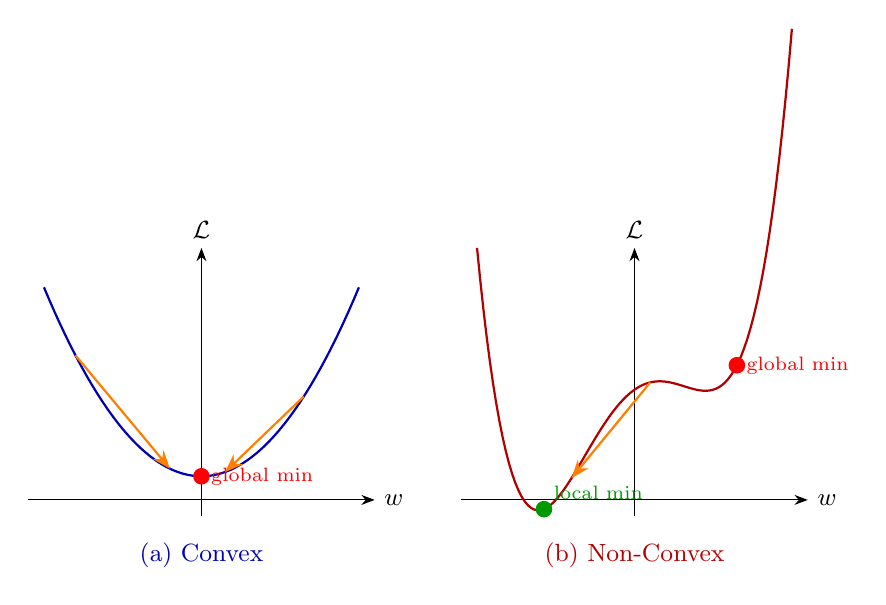
\begin{tikzpicture}[>=Stealth, scale=1.0]
  %% Left: Convex
  \begin{scope}[xshift=0cm]
    \draw[->] (-2.2,0) -- (2.2,0) node[right,font=\small]{$w$};
    \draw[->] (0,-0.2) -- (0,3.2) node[above,font=\small]{$\mathcal{L}$};
    \draw[thick,blue!70!black,domain=-2:2,samples=60]
      plot (\x, {0.6*\x*\x + 0.3});
    \fill[red] (0,0.3) circle (3pt) node[right,font=\scriptsize]{global min};
    \draw[->,orange,thick] (-1.6,{0.6*1.6*1.6+0.3}) -- (-0.4,{0.6*0.4*0.4+0.3});
    \draw[->,orange,thick] (1.3,{0.6*1.3*1.3+0.3}) -- (0.3,{0.6*0.3*0.3+0.3});
    \node[font=\small,blue!70!black] at (0,-0.7) {(a) Convex};
  \end{scope}
  %% Right: Non-convex
  \begin{scope}[xshift=5.5cm]
    \draw[->] (-2.2,0) -- (2.2,0) node[right,font=\small]{$w$};
    \draw[->] (0,-0.2) -- (0,3.2) node[above,font=\small]{$\mathcal{L}$};
    \draw[thick,red!70!black,domain=-2:2,samples=100]
      plot (\x, {0.5*\x*\x*\x*\x - 1.2*\x*\x + 0.7*\x + 1.4});
    \fill[green!60!black] (-1.15,{0.5*1.15^4 - 1.2*1.15^2 - 0.7*1.15 + 1.4}) circle (3pt)
      node[above right,font=\scriptsize]{local min};
    \fill[red] (1.3,{0.5*1.3^4 - 1.2*1.3^2 + 0.7*1.3 + 1.4}) circle (3pt)
      node[right,font=\scriptsize]{global min};
    \draw[->,orange,thick] (0.2,{0.5*0.2^4-1.2*0.2^2+0.7*0.2+1.4})
      -- (-0.8,{0.5*0.8^4-1.2*0.8^2-0.7*0.8+1.4});
    \node[font=\small,red!70!black] at (0,-0.7) {(b) Non-Convex};
  \end{scope}
\end{tikzpicture}
\caption{Schematic loss surfaces: (a) convex --- gradient descent always
  converges to the unique global minimum; (b) non-convex --- gradient descent
  may get trapped in a local minimum.  Neural network loss surfaces are
  generally non-convex.}
\label{fig:loss-surface}
\end{figure}

\begin{keyinsight}[title=Convex vs.\ Non-Convex Implications]
\begin{itemize}[noitemsep]
  \item A \textbf{convex} loss surface has a single global minimum.  Gradient
        descent with any positive learning rate is guaranteed to converge.
  \item A \textbf{non-convex} loss surface has multiple local minima and saddle
        points.  Standard gradient descent may get stuck.
  \item Neural network loss surfaces are \textbf{generally non-convex}.  This
        motivates advanced optimizers (SGD with momentum, Adam, RMSProp) and
        careful weight initialisation strategies.
\end{itemize}
\end{keyinsight}

\subsection{Effect of the Learning Rate on Gradient Descent}

The learning rate $\eta$ controls the step size along the negative gradient
direction.  From the discussion in the session:

\begin{itemize}[noitemsep]
  \item If $\eta$ is \textbf{too large}: the update step overshoots the
        minimum, potentially causing the loss to \emph{increase} or oscillate.
  \item If $\eta$ is \textbf{too small}: convergence is very slow, and
        training may take impractically many epochs.
  \item \textbf{Gradient magnitude matters}: when gradients are very large
        (e.g.\ $\approx 97$ in the numerical example), a small $\eta$ such as
        $10^{-4}$ is necessary to keep the step size reasonable.
\end{itemize}

\begin{warningbox}[title=Exploding and Vanishing Gradients]
Two pathological regimes arise during backpropagation in deep networks:
\begin{description}[noitemsep]
  \item[Exploding gradients:] Gradients grow exponentially with depth.
        Observed in the session when $\partial\mathcal{L}/\partial V_1 \approx 97$,
        $\partial\mathcal{L}/\partial W_{11} \approx 1413$.
        Remedy: gradient clipping, careful initialisation, batch normalisation.
  \item[Vanishing gradients:] Gradients shrink exponentially with depth,
        halting learning in early layers.
        Remedy: ReLU activation (avoids sigmoid saturation), residual connections,
        careful initialisation (Xavier, He).
\end{description}
The instructor noted that these topics would be covered in the following session.
\end{warningbox}

%% =============================================================================
\section{Numerical Walk-Through: Toy IQ/CGPA Network}
\label{sec:numerical}
%% =============================================================================

\subsection{Network Architecture}

The toy dataset used throughout the session predicts salary (LPA) from IQ and
CGPA:

\begin{center}
\begin{tabular}{ccc}
\toprule
IQ ($X_1$) & CGPA ($X_2$) & LPA ($Y$) \\
\midrule
80 & 8  & 3 \\
60 & 9  & 4 \\
75 & 7  & 8 \\
127 & ?  & 11 \\
\bottomrule
\end{tabular}
\end{center}

The network has 2 input neurons, 2 hidden neurons (ReLU), and 1 output neuron
(linear).  Initial weights:

\begin{align*}
  W_{11} = 0.02,\quad W_{12} = 0.50,\quad
  W_{21} = 0.04,\quad W_{22} = -0.30,\\
  V_1 = 1.20,\quad V_2 = 0.80,\quad
  B_1 = B_2 = B_3 = 1.0.
\end{align*}

\subsection{Forward Pass (Pattern 1: $X_1=80$, $X_2=8$, $Y=3$)}

\begin{align}
  Z_1 &= 0.02\times80 + 0.50\times8 + 1 = 1.6 + 4.0 + 1 = 6.6,\\
  H_1 &= \text{ReLU}(6.6) = 6.6,\\
  Z_2 &= 0.04\times80 + (-0.30)\times8 + 1 = 3.2 - 2.4 + 1 = 1.8,\\
  H_2 &= \text{ReLU}(1.8) = 1.8,\\
  \hat{y} &= 1.20\times6.6 + 0.80\times1.8 + 1.0 = 7.92 + 1.44 + 1.0 = 10.36,\\
  \mathcal{L} &= (3 - 10.36)^{2} = 54.17.
\end{align}

\subsection{Backward Pass (Selected Gradients)}

\begin{align}
  \pd{\mathcal{L}}{\hat{y}} &= 2(10.36 - 3) = 14.72,\\
  \pd{\mathcal{L}}{V_1} &= 14.72\times 6.6 = 97.15,\\
  \pd{\mathcal{L}}{V_2} &= 14.72\times 1.8 = 26.50,\\
  \pd{\mathcal{L}}{B_3} &= 14.72,\\
  \pd{\mathcal{L}}{W_{11}} &= 14.72\times1.2\times1.0\times80 = 1412.9.
\end{align}

The large gradient values (97, 26, 1413) motivate the choice of
$\eta = 10^{-4}$.

\subsection{Weight Update and Iteration 2}

\begin{align}
  V_1^{\mathrm{new}} &= 1.20 - 10^{-4}\times97.15 \approx 1.190,\\
  V_2^{\mathrm{new}} &= 0.80 - 10^{-4}\times26.50 \approx 0.797,\\
  B_3^{\mathrm{new}} &= 1.00 - 10^{-4}\times14.72 \approx 0.9985,\\
  W_{11}^{\mathrm{new}} &= 0.02 - 10^{-4}\times1412.9 \approx -0.121.
\end{align}

After updating all nine parameters and repeating the forward pass:

\begin{equation}
  \hat{y}^{(2)} \approx 0.99,\qquad
  \mathcal{L}^{(2)} = (3 - 0.99)^{2} \approx 4.04.
\end{equation}

A reduction from 54.17 to 4.04 --- a factor of $\approx\!13\times$ improvement
--- in \emph{one} gradient step.

\begin{example}[title=Interpreting Weight Direction Change]
A student asked why all weights decreased in iteration~1.  The instructor
explained with reference to the loss surface: the sign of the weight update
depends on which side of the minimum the current weight value lies.
\begin{itemize}[noitemsep]
  \item If we are on the \emph{right} side of the minimum (positive gradient),
        the weight decreases.
  \item If we are on the \emph{left} side (negative gradient), the weight
        increases.
\end{itemize}
Since only one iteration was shown, and the initialisation happened to place
all parameters on the right side, all weights decreased.  In general both
directions are possible.
\end{example}

%% =============================================================================
\section{PyTorch Implementation}
\label{sec:pytorch}
%% =============================================================================

\subsection{Version 1: Manual Backpropagation}
\label{sub:manual-backprop}

The instructor implemented the complete forward and backward passes from
scratch in PyTorch, using only scalar tensor arithmetic (no \texttt{nn.Module},
no built-in loss, no optimizer).

\subsubsection{Data and Weight Initialisation}

\begin{verbatim}
import torch

# Dataset tensors
X = torch.tensor([[80., 8.], [60., 9.], [75., 7.], [127., 12.]])
Y = torch.tensor([[3.], [4.], [8.], [11.]])

# Weight initialisation (matching the numerical example)
W11 = torch.tensor(0.02); W12 = torch.tensor(0.50)
W21 = torch.tensor(0.04); W22 = torch.tensor(-0.30)
V1  = torch.tensor(1.20); V2  = torch.tensor(0.80)
B1  = torch.tensor(1.0);  B2  = torch.tensor(1.0);  B3 = torch.tensor(1.0)

lr     = 1e-4
epochs = 2
loss_history = []
\end{verbatim}

\subsubsection{Activation Functions (Defined from Scratch)}

\begin{verbatim}
def relu(x):
    return torch.where(x > 0, x, torch.tensor(0.0))

def relu_derivative(x):
    return torch.where(x > 0, torch.tensor(1.0), torch.tensor(0.0))
\end{verbatim}

\subsubsection{Training Loop (One Row at a Time)}

\begin{verbatim}
for epoch in range(epochs):
    total_loss = 0.0
    for i in range(len(X)):
        X1, X2 = X[i, 0], X[i, 1]
        target  = Y[i, 0]

        # ─── Forward pass ───────────────────────────────────────────
        Z1   = W11*X1 + W12*X2 + B1
        H1   = relu(Z1)
        Z2   = W21*X1 + W22*X2 + B2
        H2   = relu(Z2)
        yhat = V1*H1 + V2*H2 + B3
        loss = (target - yhat)**2
        total_loss += loss

        # ─── Backward pass ──────────────────────────────────────────
        DL_Dyhat = 2*(yhat - target)
        DV1  = DL_Dyhat * H1
        DV2  = DL_Dyhat * H2
        DB3  = DL_Dyhat

        DL_DH1 = DL_Dyhat * V1
        DH1_DZ1 = relu_derivative(Z1)
        DW11 = DL_DH1 * DH1_DZ1 * X1
        DW12 = DL_DH1 * DH1_DZ1 * X2
        DB1  = DL_DH1 * DH1_DZ1

        DL_DH2 = DL_Dyhat * V2
        DH2_DZ2 = relu_derivative(Z2)
        DW21 = DL_DH2 * DH2_DZ2 * X1
        DW22 = DL_DH2 * DH2_DZ2 * X2
        DB2  = DL_DH2 * DH2_DZ2

        # ─── Parameter update ────────────────────────────────────────
        W11 -= lr * DW11;  W12 -= lr * DW12
        W21 -= lr * DW21;  W22 -= lr * DW22
        V1  -= lr * DV1;   V2  -= lr * DV2
        B1  -= lr * DB1;   B2  -= lr * DB2;  B3 -= lr * DB3

    loss_history.append(total_loss.item())
    print(f"Epoch {epoch+1}: loss = {total_loss.item():.4f}")
\end{verbatim}

\subsection{Version 2: PyTorch Autograd}
\label{sub:autograd}

In the second version the instructor introduced \texttt{torch.autograd},
PyTorch's automatic differentiation engine.  By setting
\texttt{requires\_grad=True} on each parameter tensor, PyTorch automatically
builds a computation graph during the forward pass and computes all gradients
via a single call to \texttt{loss.backward()}.

\begin{verbatim}
# Weights with gradient tracking
W11 = torch.tensor(0.02, requires_grad=True)
W12 = torch.tensor(0.50, requires_grad=True)
# ... (same for all parameters) ...

# Inside training loop:
yhat = V1*H1 + V2*H2 + B3
loss = (target - yhat)**2

loss.backward()   # Autograd computes ALL gradients

with torch.no_grad():
    W11 -= lr * W11.grad
    # ... update all parameters ...

# Zero gradients before next iteration
W11.grad.zero_()
# ... zero all grads ...
\end{verbatim}

\begin{keyinsight}[title=Manual vs.\ Autograd Verification]
A key pedagogical goal of the session was to show that the gradients computed
manually match those computed by Autograd to numerical precision.  This
verification confirms that the chain-rule derivation in
\cref{sec:backprop} is correct and builds trust in the Autograd abstraction
before using it blindly in future sessions.
\end{keyinsight}

\subsection{Weight Initialisation Strategies}
\label{sub:weight-init}

A student asked whether the initial weight values affect convergence.  The
instructor confirmed that they do and previewed the following techniques
(to be covered in depth in later sessions):

\begin{table}[htbp]
\centering
\caption{Common weight initialisation strategies.}
\label{tab:weight-init}
\begin{tabularx}{\linewidth}{lXX}
\toprule
\textbf{Method} & \textbf{Distribution} & \textbf{Best for} \\
\midrule
Zero init & $w = 0$ & Not recommended (symmetry breaking failure) \\
Random uniform & $w \sim \mathcal{U}(-1,1)$ & Simple, but may cause vanishing/exploding gradients \\
Xavier (Glorot) & $w \sim \mathcal{U}\!\left(-\sqrt{6/(n_\text{in}+n_\text{out})},\sqrt{6/(n_\text{in}+n_\text{out})}\right)$ & Sigmoid/Tanh activations \\
He (Kaiming) & $w \sim \mathcal{N}(0, 2/n_\text{in})$ & ReLU activations \\
\bottomrule
\end{tabularx}
\end{table}

%% =============================================================================
\section{Activation Functions: From Step to Differentiable}
\label{sec:activations}
%% =============================================================================

\subsection{The Sigmoid Function}

The logistic sigmoid was historically the first differentiable nonlinearity
used to replace the perceptron step function:

\begin{equation}
  \sigma(x) = \frac{1}{1 + e^{-x}},\qquad
  \sigma'(x) = \sigma(x)\bigl(1 - \sigma(x)\bigr).
  \label{eq:sigmoid}
\end{equation}

The derivative $\sigma'(x)$ is non-zero for all $x \in \mathbb{R}$, which
enables error propagation.  However, for $|x| \gg 1$ the derivative is
very close to zero (saturation), leading to the \emph{vanishing gradient}
problem in deep networks.

\subsection{The Rectified Linear Unit (ReLU)}

\begin{equation}
  \text{ReLU}(x) = \max(0, x) =
  \begin{cases} x & x > 0,\\ 0 & x \leq 0. \end{cases}
  \label{eq:relu}
\end{equation}

ReLU has become the default activation in modern deep learning because:
\begin{enumerate}[noitemsep]
  \item Its derivative is 1 for all positive inputs (no gradient saturation on
        the positive side).
  \item It is computationally cheap.
  \item It empirically works better than sigmoid in most deep architectures.
\end{enumerate}

The instructor stressed that \emph{any} differentiable nonlinear function can
be used --- the choice is guided by empirical performance and specific task
requirements.

\subsection{Comparison of Activation Functions}

\begin{table}[htbp]
\centering
\caption{Properties of activation functions discussed in the session.}
\label{tab:activations}
\begin{tabularx}{\linewidth}{lXXXX}
\toprule
\textbf{Function} & \textbf{Range} & \textbf{Differentiable} & \textbf{Vanishing Grad?} & \textbf{Common Use} \\
\midrule
Signum (step) & $\{-1,+1\}$ & No (at 0) & N/A & Perceptron \\
Sigmoid & $(0,1)$ & Yes & Yes (deep nets) & Binary output \\
Tanh & $(-1,1)$ & Yes & Yes (deep nets) & RNN gates \\
ReLU & $[0,\infty)$ & No (at 0) & No (positive side) & Hidden layers \\
Leaky ReLU & $(-\infty,\infty)$ & Yes & No & Hidden layers \\
\bottomrule
\end{tabularx}
\end{table}

%% =============================================================================
\section{Summary and Conclusion}
\label{sec:summary}
%% =============================================================================

\subsection{Key Concepts Covered}

Session~06 completed the theoretical backbone of feedforward ANNs.  The
following core ideas were developed:

\begin{enumerate}[label=\arabic*.,noitemsep]
  \item \textbf{Hard problem vs.\ hard learning problem.}  The hard problem
        (linear inseparability) is solved by adding hidden layers.  The hard
        learning problem (no target outputs for hidden units) is solved by
        backpropagation.

  \item \textbf{Role of differentiability.}  Replacing the step function with
        a differentiable activation (sigmoid, ReLU) is the critical enabler of
        backpropagation.  Without a non-zero derivative, the error signal
        cannot be propagated backward.

  \item \textbf{Generalized delta rule.}  Backpropagation is a direct
        generalization of the single-layer delta rule.  The update formula
        $\Delta w = \eta \cdot \delta \cdot \text{input}$ holds at every layer,
        with $\delta$ computed via the chain rule.

  \item \textbf{MSE loss.}  The squared error $(y - \hat{y})^2$ and its mean
        over the dataset provide a differentiable training objective whose
        gradient is $2(\hat{y}-y)$.

  \item \textbf{Convex vs.\ non-convex surfaces.}  Neural network loss
        landscapes are non-convex.  Gradient descent behavior (weight
        increase or decrease) depends on which side of a minimum the current
        parameters lie.

  \item \textbf{Learning rate selection.}  A learning rate of $\eta = 10^{-4}$
        was necessary because the raw gradients were of order $10^2$--$10^3$.
        Poor learning rate choice leads to exploding gradients (too large) or
        extremely slow convergence (too small).

  \item \textbf{PyTorch Autograd.}  The automatic differentiation system
        eliminates the need to hand-code gradients.  Its results match manual
        derivations exactly, confirming correctness of the theory.
\end{enumerate}

\subsection{Formulae Reference Card}

\begin{keyinsight}[title=Essential Backpropagation Formulae]
\begin{align*}
  &\textbf{Output layer error signal:}
  &\deltak &= (b_k - \sko)\,f'(\xko)\\
  &\textbf{Output layer weight update:}
  &\Delta\wkj &= \eta\,\deltak\,\sho\\
  &\textbf{Hidden layer error signal:}
  &\deltajh &= f'(\xho)\sum_{k=1}^{K}\deltak\,\wkj\\
  &\textbf{Hidden layer weight update:}
  &\Delta\wji &= \eta\,\deltajh\,a_i\\
  &\textbf{General update:}
  &\theta &\leftarrow \theta - \eta\,\pd{\mathcal{L}}{\theta}
\end{align*}
\end{keyinsight}

\subsection{Looking Ahead}

The next session will continue from this foundation by examining:

\begin{itemize}[noitemsep]
  \item Vanishing and exploding gradient problems in depth.
  \item Weight initialisation techniques (Xavier, He).
  \item Batch normalisation and its role in stabilising training.
  \item Advanced optimizers beyond plain SGD.
\end{itemize}

The instructor's advice to students: practice the PyTorch Colab notebook
independently, vary the learning rate and initial weights, and observe the
effect on loss convergence.  A firm grasp of this two-layer example is the
foundation for understanding any deeper architecture.

\vspace{1cm}
\hrule
\vspace{0.4cm}
{\small
\textbf{Source materials:}
Transcript: \texttt{session06\_transcript.vtt};
Visual extraction: \texttt{session06\_visual\_extraction.md};
Slide deck: \texttt{02-DL-NNIntro} (slides 50--87/87).
Reference: B.\ Yegnanarayana, \textit{Artificial Neural Networks}, PHI,
New Delhi, 1999.
}

\end{document}
